\chapter{Theoretical background}
\section{Interaction of Radiation with Matter}\label{RadMatter}
In the following, we will derive the necessary equations describing how a quantized field interacts with matter within the framework of the second quantization. We will assume the final quantized form of the vector potential given by
\begin{equation} \label{quantized}
	\vec{A}(\vec{r},t) = \sum_{\vec{k},\lambda} \sqrt{\frac{2\pi\hbar c^2}{\omega_k V}} \bigg(a_{k,\lambda}\vec{e}_{\vec{k},\lambda}\text{e}^{i(\vec{k}\cdot \vec{r})-i\omega_k t}+a_{\vec{k,\lambda}}^\dagger\vec{e}_{\vec{k},\lambda}^*\text{e}^{-i(\vec{k}\cdot \vec{r})+i\omega_k t}\bigg)
\end{equation}
We now consider a non-relativistic system of charged particles interacting with the electromagnetic field. In this thesis, we will consider a two-particle system, but in this section, we generalize the results to any integer of particles denoted by the subscript $i$. The interaction will enable the system to emit and absorb photons. We start with the usual Hamiltonian describing the many-body system given by $H_0(\vec{r}_i),\vec{p_i}$ with no field. We introduce a field and do the following substitution 
\begin{equation} \label{substi}
	\vec{p}_i \rightarrow \vec{p}_i - \frac{e_i}{c}\vec{A}(\vec{r}_i),
\end{equation}
where $e_i$ is the charge of the $i$'th particle and $c$ is the speed of light. This leads to a new Hamiltonian, which now depends on the field variables
\begin{equation} \label{withfield}
	H_0 \rightarrow H_0' = H_0 \left( \vec{r}_i,\vec{p}_i-\frac{e_i}{c}\vec{A}(\vec{r}_i)\right) + \sum_i e_i \phi(\vec{r}_i),
\end{equation}
where the last term in equation \eqref{withfield} is the potential energy. We now introduce the radiation gauge choice, which is purely conventional and any other choice of gauge will result in the same equations, albeit more difficult. The radiation gauge is given by
\begin{equation} \label{RadiationGauge}
	\vec{\nabla}\cdot \vec{A} = \phi = 0,
\end{equation}
and the non-relativistic Hamiltonian of the system describing the interaction with the radiation field is given by
\begin{equation} \label{Rad}
	H = \sum_i \frac{1}{2m_i}\left( \vec{p}-\frac{e_i}{c}\vec{A}(\vec{r}_i)\right)^2,
\end{equation}
where $\vec{A}(\vec{r}_i)$ is equation \eqref{quantized} at point $\vec{r}_i$. We assumed the interaction between particles depends on their coordinates, so the minimal inclusion of the electromagnetic field affects only the kinetic part. This is a fair approximation in the non-relativistic limit and does not account for velocity-dependant interactions such as spin-orbit\footnote{One could add a spin-orbit term to the non-relativistic approach, but this is not necessary for our calculations later}. 
The electromagnetic interaction is relatively weak, and its strength is given by the fine structure constant, $\alpha = e^2/(\hbar c)$. Generally speaking, this interaction can be taken into account in the lowest non-vanishing order of perturbation theory. We expand \eqref{Rad} and keep only the linear terms
\begin{equation} \label{RadLin}
	H^{(1)} = -\sum_i \frac{e_i}{2m_i c} (\vec{p}_i\cdot \vec{A}(\vec{r}_i)+\vec{A}(\vec{r}_i)\cdot \vec{p}_i),
\end{equation}
where the $(1)$ represents the first non-vanishing order. Due to our choice of gauge equation \eqref{RadiationGauge} the two terms in \eqref{RadLin} commute and we are left with
\begin{equation} \label{RadiationHamil}
	H^{(1)} = - \sum_i \frac{e_i}{m_i c} \vec{A}(\vec{r}_i,t)\vec{p}_i.
\end{equation}
For the type of problems, we will be solving in \ref{sec:PionPhotoproduction}, we will be working mainly with one charged particle, and we can ignore the sum in \eqref{RadiationHamil}.
\section{Density of States}\label{sec:densityofstates}
As mentioned in section \ref{RadMatter} the electromagnetic interaction strength is related to the fine structure constant. In section \ref{sec:PionPhotoproduction}, we want to do perturbation theory to get an expression for the total cross-section as a function of energy which the relatively weak fine structure constant allows. From perturbation theory, the transition rate is described by Fermi's golden rule given by
\begin{equation} \label{FermiGolden}
	\text{d}\omega = \frac{2\pi}{\hbar}\abs{\mathcal{M}}^2 \text{d}\rho,
\end{equation}
where the matrix element $\mathcal{M}$ is the subject in section \ref{sec:PionPhotoproduction} and $\text{d}\rho$ is the density of states in the final states. In this section, we will derive general results of the density of states in the non-relativistic and relativistic limits. The density of states is defined by
\begin{marginfigure}
	\centering
	

\tikzset{every picture/.style={line width=0.75pt}} %set default line width to 0.75pt        

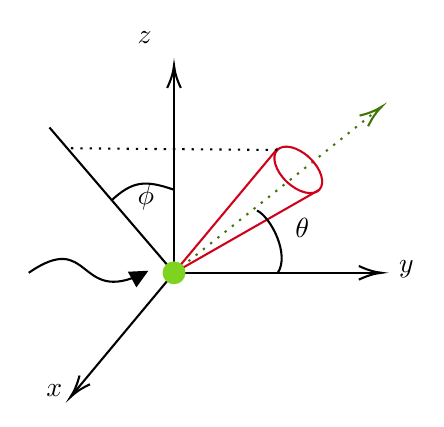
\begin{tikzpicture}[x=0.75pt,y=0.75pt,yscale=-1,xscale=1]
%uncomment if require: \path (0,362); %set diagram left start at 0, and has height of 362

%Straight Lines [id:da8075674552034334] 
\draw    (270,180) -- (210,110) ;
%Straight Lines [id:da1934453842044379] 
\draw [color={rgb, 255:red, 65; green, 117; blue, 5 }  ,draw opacity=1 ] [dash pattern={on 0.84pt off 2.51pt}]  (270,180) -- (368.44,101.25) ;
\draw [shift={(370,100)}, rotate = 141.34] [color={rgb, 255:red, 65; green, 117; blue, 5 }  ,draw opacity=1 ][line width=0.75]    (10.93,-3.29) .. controls (6.95,-1.4) and (3.31,-0.3) .. (0,0) .. controls (3.31,0.3) and (6.95,1.4) .. (10.93,3.29)   ;
%Straight Lines [id:da551977907100426] 
\draw [color={rgb, 255:red, 208; green, 2; blue, 27 }  ,draw opacity=1 ]   (270,180) -- (340,140) ;
%Straight Lines [id:da13834667273930523] 
\draw [color={rgb, 255:red, 208; green, 2; blue, 27 }  ,draw opacity=1 ]   (270,180) -- (320,120) ;
%Straight Lines [id:da575178064615293] 
\draw    (270,180) -- (270,82) ;
\draw [shift={(270,80)}, rotate = 90] [color={rgb, 255:red, 0; green, 0; blue, 0 }  ][line width=0.75]    (10.93,-3.29) .. controls (6.95,-1.4) and (3.31,-0.3) .. (0,0) .. controls (3.31,0.3) and (6.95,1.4) .. (10.93,3.29)   ;
%Straight Lines [id:da30763782233069703] 
\draw    (270,180) -- (368,180) ;
\draw [shift={(370,180)}, rotate = 180] [color={rgb, 255:red, 0; green, 0; blue, 0 }  ][line width=0.75]    (10.93,-3.29) .. controls (6.95,-1.4) and (3.31,-0.3) .. (0,0) .. controls (3.31,0.3) and (6.95,1.4) .. (10.93,3.29)   ;
%Straight Lines [id:da016368323591563816] 
\draw    (270,180) -- (221.28,238.46) ;
\draw [shift={(220,240)}, rotate = 309.81] [color={rgb, 255:red, 0; green, 0; blue, 0 }  ][line width=0.75]    (10.93,-3.29) .. controls (6.95,-1.4) and (3.31,-0.3) .. (0,0) .. controls (3.31,0.3) and (6.95,1.4) .. (10.93,3.29)   ;
%Curve Lines [id:da6672149281430028] 
\draw    (200,180) .. controls (230.55,158.88) and (223.07,196.06) .. (255.12,180.32) ;
\draw [shift={(257.67,179)}, rotate = 151.5] [fill={rgb, 255:red, 0; green, 0; blue, 0 }  ][line width=0.08]  [draw opacity=0] (8.93,-4.29) -- (0,0) -- (8.93,4.29) -- cycle    ;
%Flowchart: Connector [id:dp12078467552802752] 
\draw  [color={rgb, 255:red, 126; green, 211; blue, 33 }  ,draw opacity=1 ][fill={rgb, 255:red, 126; green, 211; blue, 33 }  ,fill opacity=1 ] (265,180) .. controls (265,177.24) and (267.24,175) .. (270,175) .. controls (272.76,175) and (275,177.24) .. (275,180) .. controls (275,182.76) and (272.76,185) .. (270,185) .. controls (267.24,185) and (265,182.76) .. (265,180) -- cycle ;
%Shape: Ellipse [id:dp45046333760686075] 
\draw  [color={rgb, 255:red, 208; green, 2; blue, 27 }  ,draw opacity=1 ] (319.75,120.83) .. controls (322.77,117.63) and (329.76,119.33) .. (335.35,124.63) .. controls (340.94,129.92) and (343.03,136.8) .. (340,140) .. controls (336.97,143.2) and (329.99,141.49) .. (324.4,136.2) .. controls (318.8,130.91) and (316.72,124.02) .. (319.75,120.83) -- cycle ;
%Straight Lines [id:da9664046710126799] 
\draw  [dash pattern={on 0.84pt off 2.51pt}]  (319.75,120.83) -- (220,120) ;
%Curve Lines [id:da6106413145156059] 
\draw    (310,150) .. controls (316.83,153.33) and (325.83,171.33) .. (320,180) ;
%Curve Lines [id:da19983569644229238] 
\draw    (240,145) .. controls (249.83,136) and (255.83,135) .. (270,140) ;

% Text Node
\draw (251,62.4) node [anchor=north west][inner sep=0.75pt]    {$z$};
% Text Node
\draw (377,172.4) node [anchor=north west][inner sep=0.75pt]    {$y$};
% Text Node
\draw (207,232.4) node [anchor=north west][inner sep=0.75pt]    {$x$};
% Text Node
\draw (327,152.4) node [anchor=north west][inner sep=0.75pt]    {$\theta $};
% Text Node
\draw (251,136.4) node [anchor=north west][inner sep=0.75pt]    {$\phi $};


\end{tikzpicture}
	\caption{Differential cross section and the solid angle $\Omega_q$ (red cone).}
	\label{fig:diffcross}
\end{marginfigure}
\begin{equation} \label{DensityOfStates}
	\rho(E) = \frac{\text{d}n(E)}{\text{d}E},
\end{equation}
where $n(E)$ is the number of states with energy $E$. Consider the number of states within the momentum space volume
\begin{equation} \label{momspace}
	\text{d}^3\vec{p} = p^2 \text{d}p \, \text{d}\Omega_q,
\end{equation}
where the subscript $q$ is used to empathize momentum space. We will use this notation throughout the thesis. Equation \eqref{momspace} corresponds to the momenta with magnitude from $p$ to $p+\text{d}p$ and within a cone of solid angle $\text{d}\Omega_q$. This is illustrated in figure \ref{fig:diffcross}. We use the solutions to the Schrödinger equation for a particle confined in a large volume with periodic boundary conditions are travelling waves. This leads to the following expression
\begin{equation} \label{densityrho}
	\rho(p) \, \text{d}\rho = \left( \frac{L}{2\pi\hbar}\right)^3 \text{d}^3 \vec{p} = \frac{V}{(2\pi\hbar)^3} p^2 \, \text{d}p \, \text{d}\Omega_q.
\end{equation}
In section \ref{sec:PionPhotoproduction}, we are interested in the number of possible final states with energy in the range between $E_f$ and $E_f + \text{d}E_f$ so we express \eqref{densityrho} in terms of energy. This is given by
\begin{equation} \label{densityenergy}
	\rho(E_f) = \frac{V p_f^2}{(2\pi \hbar)^3} \frac{\text{d}p_f}{\text{d}E_f} \, \text{d}\Omega_q.
\end{equation}
This is the final expression non-relativistically. However, we want to generalize this result to account for relativistic effects since we have yet to determine what relativistic regime will dominate the process. For a general pion photoproduction process, we can write
\begin{equation} \label{twobody}
	N + \gamma \rightarrow N+\pi,
\end{equation}
where $N$ is the nucleon. The final state energy is then given by \cite{Kernebog}
\begin{equation} \label{Ef}
	E_f = E_N + E_\pi = \sqrt{p_f^2 c^2 +m_N^2c^4} + \sqrt{p_f^2c^2 + m^2_\pi c^4}.
\end{equation}
We now change the notation to match the variables used later in section \ref{sec:PionPhotoproduction} and write the final state momentum $p_f$ in terms of the wave number $q$. 


From conservation of energy, we get the following expression for the energy of the relative pion-nucleon motion denoted $E_q$. 
\begin{equation} \label{Eq}
	E_q = \sqrt{m_N^2 c^4+(\hbar c)^2q^2} + \sqrt{m_\pi c^4+(\hbar c)^2 q^2}-m_N c^2-m_\pi c^2.
\end{equation}

\begin{marginfigure}
	\centering
	

\tikzset{every picture/.style={line width=0.75pt}} %set default line width to 0.75pt        

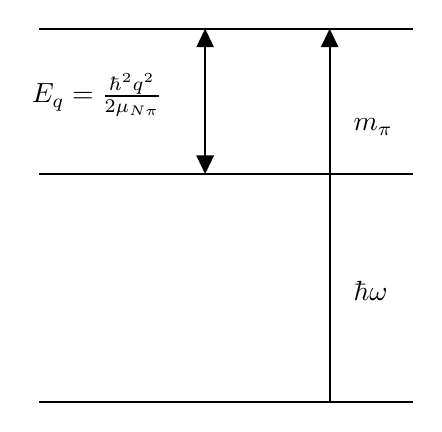
\begin{tikzpicture}[x=0.75pt,y=0.75pt,yscale=-1,xscale=1]
	%uncomment if require: \path (0,300); %set diagram left start at 0, and has height of 300
	
	%Straight Lines [id:da9050164165880492] 
	\draw    (210,200) -- (390,200) ;
	%Straight Lines [id:da595724624922532] 
	\draw    (210,90) -- (390,90) ;
	%Straight Lines [id:da8326738532712242] 
	\draw    (210,20) -- (390,20) ;
	%Straight Lines [id:da4515077860512252] 
	\draw    (350,200) -- (350,23) ;
	\draw [shift={(350,20)}, rotate = 90] [fill={rgb, 255:red, 0; green, 0; blue, 0 }  ][line width=0.08]  [draw opacity=0] (8.93,-4.29) -- (0,0) -- (8.93,4.29) -- cycle    ;
	%Straight Lines [id:da5226155750538098] 
	\draw    (290,87) -- (290,23) ;
	\draw [shift={(290,20)}, rotate = 90] [fill={rgb, 255:red, 0; green, 0; blue, 0 }  ][line width=0.08]  [draw opacity=0] (8.93,-4.29) -- (0,0) -- (8.93,4.29) -- cycle    ;
	\draw [shift={(290,90)}, rotate = 270] [fill={rgb, 255:red, 0; green, 0; blue, 0 }  ][line width=0.08]  [draw opacity=0] (8.93,-4.29) -- (0,0) -- (8.93,4.29) -- cycle    ;
	
	% Text Node
	\draw (360,140) node [anchor=north west][inner sep=0.75pt]    {$\hbar \omega $};
	% Text Node
	\draw (360,62) node [anchor=north west][inner sep=0.75pt]    {$m_{\pi }$};
	% Text Node
	\draw (205,40) node [anchor=north west][inner sep=0.75pt]    {$E_{q} =\frac{\hbar ^{2} q^{2}}{2\mu _{N\pi }}$};
	
	
\end{tikzpicture}
	\caption{Energy diagram of the system. Here $\mu_{N\pi}$ is the reduced mass of the pion-nucleon system}
	\label{fig:qenergy}
\end{marginfigure}
Looking at \eqref{densityenergy}, we want to get an expression for the final state momentum in terms of the wave number. The density of states around $\vec{q}$ is given by
\begin{equation} \label{DensityEQ}
	\text{d}\rho_f = \frac{Vq}{(2\pi)^3}\frac{1}{2}\frac{\text{d}q^2}{\text{d}E_q} \text{d}\Omega_q.
\end{equation}
We now solve for $(\hbar c)^2q^2$ in \eqref{Eq}, which yields the following result\footnote{It is also possible to use the approximation that $\sqrt{x^2+y^2}\simeq 0.96x+0.4y$ giving an error of only $4\%$.}
\begin{equation} \label{hbarc-q}
	(\hbar c)^2 q^2 = \frac{E_q(E_q+2m_N c^2)(E_q+2m\pi c^2)(E_q+2m_N c^2+2m_\pi c^2)}{4(E_q+m_N c^2+m_\pi c^2)^2},
\end{equation}
and we are now able to calculate the derivative of equation \eqref{hbarc-q}
\begin{equation}\begin{split} \label{derivative}
		(\hbar c)^2\frac{\text{d}q^2}{\text{d}E_q} &= \frac{(E_q^2+2E_q m_N c^2+2m_N^2 c^4+2E_q m_\pi c^2+2m_N m_\pi c^4)}{2(E_q+m_N c^2+m_\pi c^2)^3} \\
		& \, \times \frac{(E_q^2+2E_q m_N c^2 +2m_\pi^2 c^4 +2E_q m_\pi c^2+2m_N m_\pi c^4)}{2(E_q+m_N c^2+m_\pi c^2)^3},
	\end{split}
\end{equation} 
which yields the final expression for the relativistic density of states by plugging equation \eqref{derivative} into equation \eqref{DensityEQ}. Non-relativistically, the density of states in terms of $E_q$ and $q$ is given by the following using 
\begin{equation}\label{nonreladensity}
	\text{d}\rho = \frac{Vq\mu_{N_\pi}}{(2\pi)^3\hbar^2} \text{d}\,\Omega_q
\end{equation}